\lohead{Julian Wolf}
\chapter{Elektronik und Mechanik}
\label{sec:elektronik-und-mechanik}

\section{Anforderung Elektronik Variante 1}
\subsection{Aktoren}
Die Anforderungen der Aktoren im Elektrischen Teil, bestehen darin ein Förderband und eine Drehplatte zu drehen. Für beide Anwendungen werden Motoren mit einem hohen Drehmoment und einer niedrigen Drehzahl benötigt. Weiters dürfen sich die Motoren nicht drehen, wenn sie nicht angesteuert werden.
Zur Positionierung, Befestigung und durchführung anderer linearer Bewegungen werden weiteres Hubmagnete inf Form von Zylindermagneten benötigt. Diese Hubmagnete haben die Aufgabe Futterbeutel zu verschieben, zu positionieren, festzuhalten und einen Scherenhebel zum öffnen der Futterbeutel zu betätigen.  
\subsection{Sensoren}
Die Anforderung der Sensoren im Elektrischen Teil, bestehen darin erkennen zu können, ob ein Objekt vor ihnen steht. Dadurch kann überprüft werden, ob Futterschüsseln und Futterbeutel and der richtigen Stelle stehen, mögliche Fehler erkannt werdn und Zählungen der Futterschüsseln durchgeführt werden, damit erfasst werden kann, welche der fünf Futterschüsseln an welcher Position steht.
\subsection{Ansteuerungen}
Die Aufgabe der Ansteuerung ist es, möglichst einfach, günstig und sicher die Aktoren und Sensoren ansteuern zu können.

\section{Anforderung Elektronik Variante 2}
\subsection{Aktoren}
Die Anforderungen der Aktoren im Elektrischen Teil, bestehen darin ein Förderband und eine Drehplatte zu drehen. Für beide Anwendungen werden Motoren mit einem hohen Drehmoment und einer niedrigen Drehzahl benötigt. Weiters dürfen sich die Motoren nicht drehen, wenn sie nicht angesteuert werden.
\subsection{Sensoren}
Die Anforderung der Sensoren im Elektrischen Teil, bestehen darin erkennen zu können, ob ein Objekt vor ihnen steht. Dadurch kann überprüft werden, ob Futterschüsseln und Futterbeutel and der richtigen Stelle stehen, mögliche Fehler erkannt werdn und Zählungen der Futterschüsseln durchgeführt werden, damit erfasst werden kann, welche der fünf Futterschüsseln an welcher Position steht.
\subsection{Ansteuerungen}
Die Aufgabe der Ansteuerung ist es, möglichst einfach, günstig und sicher die Aktoren und Sensoren ansteuern zu können.

\section{Variante 1}
\subsection{Aktoren}
\subsubsection{Hubmagnete}
\begin{figure}[H] 
\begin{center}

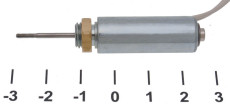
\includegraphics[width=10cm]{Bilder/Bauteile/Hubmagnet}
\caption{Hubmagnet}
\label{Hubmagnet}

\end{center}
\end{figure}
Zylinderhubmagnete bestehen aus einem zylindrischen Dauermagnetkerns. Umgeben ist dieser Magnetkern von einer Spule und einem Gehäuse, welches das ganze Konstrukt vor Festkörpern schützt. Wird an die Spule eine Spannung angelegt, fließt ein Strom durch die Spule. Dieser Strom erzeugt ein Magnetfeld was den Magnetkern anzieht oder abstößt. Durch eine gezielte übersteuerung des Magnetzylinders, kann die Kraft des Magnetfeldes kurzzeitig verstärkt werden, jedoch verhindert die erhöhte Hitzeentwicklung einen dauerhaften Betrieb im übersteuerten Zustand. Der übersteuerte Zustand wird mit einer gerngeren relativen Einschaltdauer gegenüber der Zykluszeit bewirkt. Der Strom der durch die Spule fließt kann sich durch die kurze Einschaltdauer nicht einpendeln, was der Spule erlaubt mit einem durchschnittlich höheren Strom betrieben zu werden, was zu einem stärkeren Magnetfeld und somit zu einer stärkeren Kraft führt. Die genauen Werte der Kraft zur relativen Einschaltdauer lassen sich dem Datenblatt jedes einzelnen Hubmagnetens entnehmen. Ein Vorteil von Hubmagneten ist es, dass sie in allen möglichen Formen, Hublängen, Hubkräften und Wechsel- oder Gleichspannungsbereichen verfügbar sind. Hubmagnete können auch mit 3 verschiedenen Hubzuständen erworben werden. Monostabile Hubmagnete halten sich, mithilfe einer Feder, bei stromlosen Zustand immer an der Anfangs oder Endposition. Bistabile Hubmagnete verweilen im stromlosen Zustand an ihrer aktuellen Position, also entweder im eingefahrenen oder ausgefahrenen Zustand. Tristabile Hubmagnete bleiben, wie bistabile Hubmagnete, stromlos an ihrer aktuellen Postition. Jedoch kann diese Hubmagnetart auch an einer vorgegebenen Mittelposition verweilen.

\subsubsection{Motoren}
Nach einigen Problemen und Variantenänderungen in der Mechanik, wurde die Motorenauswahl erst in Variante 2 vorgenommen, da die Auswahl für Variante 1 sinnfrei wäre.

\subsection{Sensoren}
\begin{figure}[H] 
\begin{center}

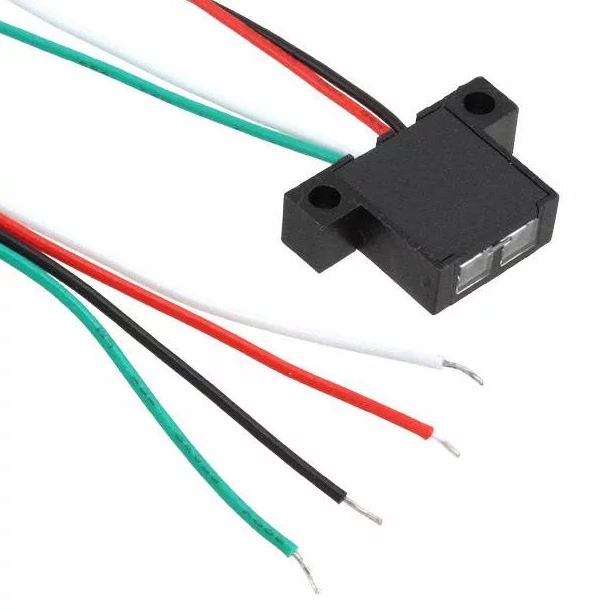
\includegraphics[width=10cm]{Bilder/Bauteile/Sensor}
\caption{Sensor}
\label{Sensor}

\end{center}
\end{figure}
Die Auswahl des Sensor für unsere Anwendung wurden von folgenden Kriterian beeinflusst: Befestingungsmöglichkeiten, Preis und zusätzlich benötigte Ansteuerungen.
Kapazitive und Induktive Näherungsschalter lassen sich einfach befestigen, sind jedoch nicht sehr günstig. Auch ist die Reichweite der Sensoren nicht sehr groß, was aber in unserer Anwendung unwichtig ist. Für diese Arten von Sensoren werden zusätzliche Ansteuerungen benötigt. Diese Ansteuerungen sind meistens teuer und benötigen zur Kommunikation mit einem Raspberry eine Schnittstelle.
Wir haben uns in diesem Anwendungsbereich für einen Optischen Näherungsschalter entschieden. Dieser beinhaltet ein fertiges Modul bestehend aus einer Infrarot LED und einem Infrarot Fototransistor. Diese Modul ist günstig und auch leicht zu befestigen. Dadurch, dass unsere Anwendung keine genaue Abstandsmessung benötigt, wird keine zusätzliche Ansteuerung benötigt. Zur Stromversorgung reichen 5V Gleichspannung mit einem laut Datenblatt berechneten Vorwiderstand. Die Auswertung erfolgt durch einen digitalen Input-Pins des Raspberrys. Sobald sich eine Reflektorfläche vor den Sensor bewegt, wird der Fototransistor niederohmig und ermöglicht somit einen Stromfluss. Dadurch liegt eine Spannung von 3,3V am Input-Pin an und wird vom Raspberry als High-Zustand angesehen. Wenn die Reflektorfläche vom Modul nicht mehr erfasst wird, sperrt der Fototransistor, der Stromfluss wird unterbunden und am Input-Pin liegen nurmehr 0V an, was als Low-Zustand angesehen wird.

\subsection{Ansteuerungen}
Da Variante 1 Nur kurze Zeit verfolgt wurde, wurden genaue Ansteuerungen für Motoren und Hubmagneten nicht herausgesucht. Der Sensor benötigt keine zusätzliche Ansteuerung

\section{Variante 2}
\subsection{Aktoren}
\subsubsection{Hubmagnete}
Für die zweite Variante werden keine Hubmagnete benötigt, da alle Befestigungen rein mechanisch erfolgen.

\subsubsection{Motoren}
\begin{figure}[H] 
\begin{center}

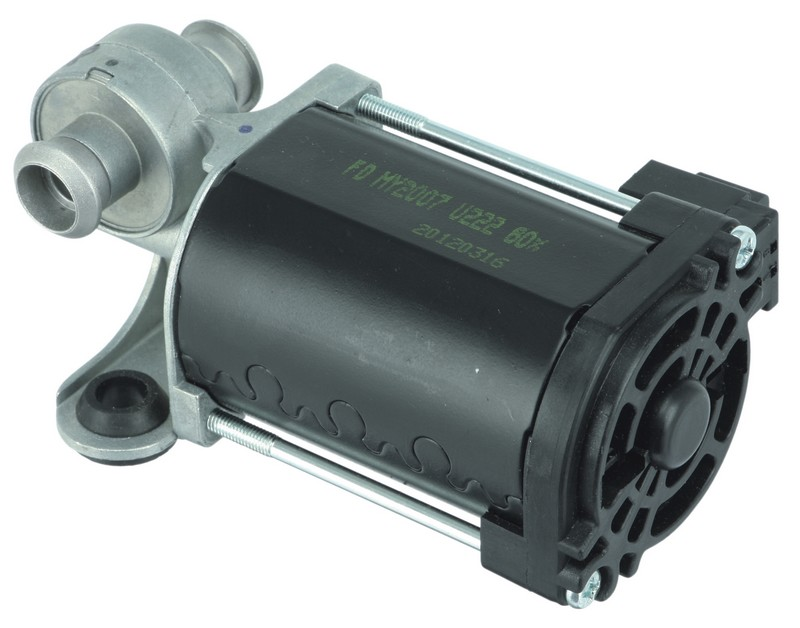
\includegraphics[width=10cm]{Bilder/Bauteile/Motor}
\caption{Motor}
\label{Motor}

\end{center}
\end{figure}
Die Motoren wurden mithilfe folgender Kriterien ausgesucht: Preis, Drehzahl, Kraft, stromloses Verhalten, Spannung.
In unserer Elektronik soll nur mit sicherer niedrieger Gleichspannung gearbeitet werden. Daher kommen nur Motoren mit einem Spannungsbereich von 0-24V in frage. Aus diesem Grund wird die Auswahl eines Asynchronmotors ausgeschlossen. Die Anwendung fordert, dass sich die Motoren im Stromlosen zustand nicht bewegen lassen. Dadurch können folgende Motorarten ausgeschlossen werden: Synchronmotoren, reine Gleichstrommotren, Schrittmotoren und Servomotoren, falls diese Motoren nicht über eine aktive Bremse verfügen. Ideal für unsere Anwendungen sind Gleichstrom-Schneckengetriebe-Motoren. Diese Motoren lassen sich aufgrund des mechanischen Auifbaus im stromlosen Zustand nicht drehen. Diese Motoren verfügen meistens auch über eine Getriebe was eine Übersetzung in eine niedrigere Drehzahl zur folge hat. Gleichzeitg wird mit diesem Getriebe auch das Drehmoment erhöht, weshalb der Motor eine höhere Kraft aufbringen kann. Zusätzlich werden Schneckengetriebemotoren in der Automobil Industrie als Scheibenwischermotoren verwendet. Daher sind diese Motoren sehr Preisgünstig zu erwerben.

\subsubsection{Lüfter}
\begin{figure}[H] 
\begin{center}

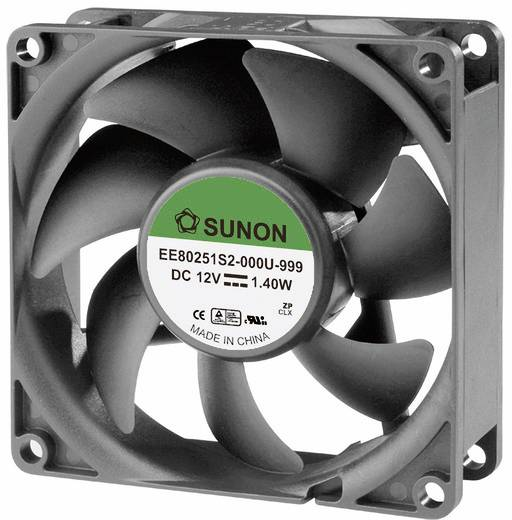
\includegraphics[width=10cm]{Bilder/Bauteile/Luefter}
\caption{Luefter}
\label{Luefter}

\end{center}
\end{figure}
Zur Kühlung des Raspberrys, wird ein externen 12V-Lüfter hergenommen, welcher einen Luftstrom um den Raspberry und den $\mu$Controller erzeugt.
\subsection{Sensoren}
Der ausgewählte Optische Sensor wurde in Variante 1 bereits beschrieben. Für genauere Informationen lesen Sie bitte in Punkt 1.3.2 nach.
Es werden zwei dieser Sensoren zur Positionierung verwendet. Der Sensor muss nur erkennen ob sich eine Reflektorfläche vor ihm befindet. Bei der Futterschüsseldrehplatte wird am Rand der Scheibe an der position jeder Futterschüssel ein Reflektorstreifen verwendet. Dadurch kann mit der Software gezählt und erkannt werden, welche Futterschüssel sich aktuell vor dem Sensor befindet. Im Futterbeutelmagazin wird der Sensor dazu verwendet um erkennen zu können ob ein Futterbeutel zum Füttern verfügbar ist. Wird vom Sensor, nach drehen des Motors, kein weiterer Futterbeutel erkannt, wird von der Software, falls nötig, ein Fehler ausgegeben und der Benutzer wird informiert. Der Reflektorstreifen wird auf der Verschlussklemme jedes Futterbeutels befestigt.
\subsection{Ansteuerung}
Der Gesamtschaltplan wurde in ProfiCad realisiert. Der Schaltplan beinhaltet die Ansteuerung der Motoren und Sensoren, sowie die Visualisierung der Verkabelung der einzelnen Elemente.
Für ein einfacheres Verständnis wird der Gesamtschaltplan in kleinere Elemente aufgeteilt und in Unterpunkten beschrieben
\subsubsection{Motoransteuerung Variante 1}
Gleichstrom Schneckengetriebemotoren haben die Fähigkeit sich in beide Richtungen zu drehen, je nach polarität der Anschlüsse. Um eine Softwaretechnische einfache Ansteuerung ermöglichen zu können, wird oft eine H-Brücke zur ansteuerung der Motoren verwendet. Diese H-Brücke besteht aus vier Transistoren. Für Motoren mit höheren Stromanforderungen werden MOSFET-Transistoren verwendet. Die Schaltung besteht aus zwei P-Kanal MOSFET T1, T2 beziehungsweise T5, T7 und aus zwei N-Kanal MOSFET T2, T4 beziehungsweise T6, T8. Die MOSFET und die Grundlegende Schaltung wurde von HIER ZITAT EINFÜGEN übernommen. Die P-Kanal 
\subsubsection{Motoransteuerung Variante 2}
\begin{figure}[H] 
\begin{center}

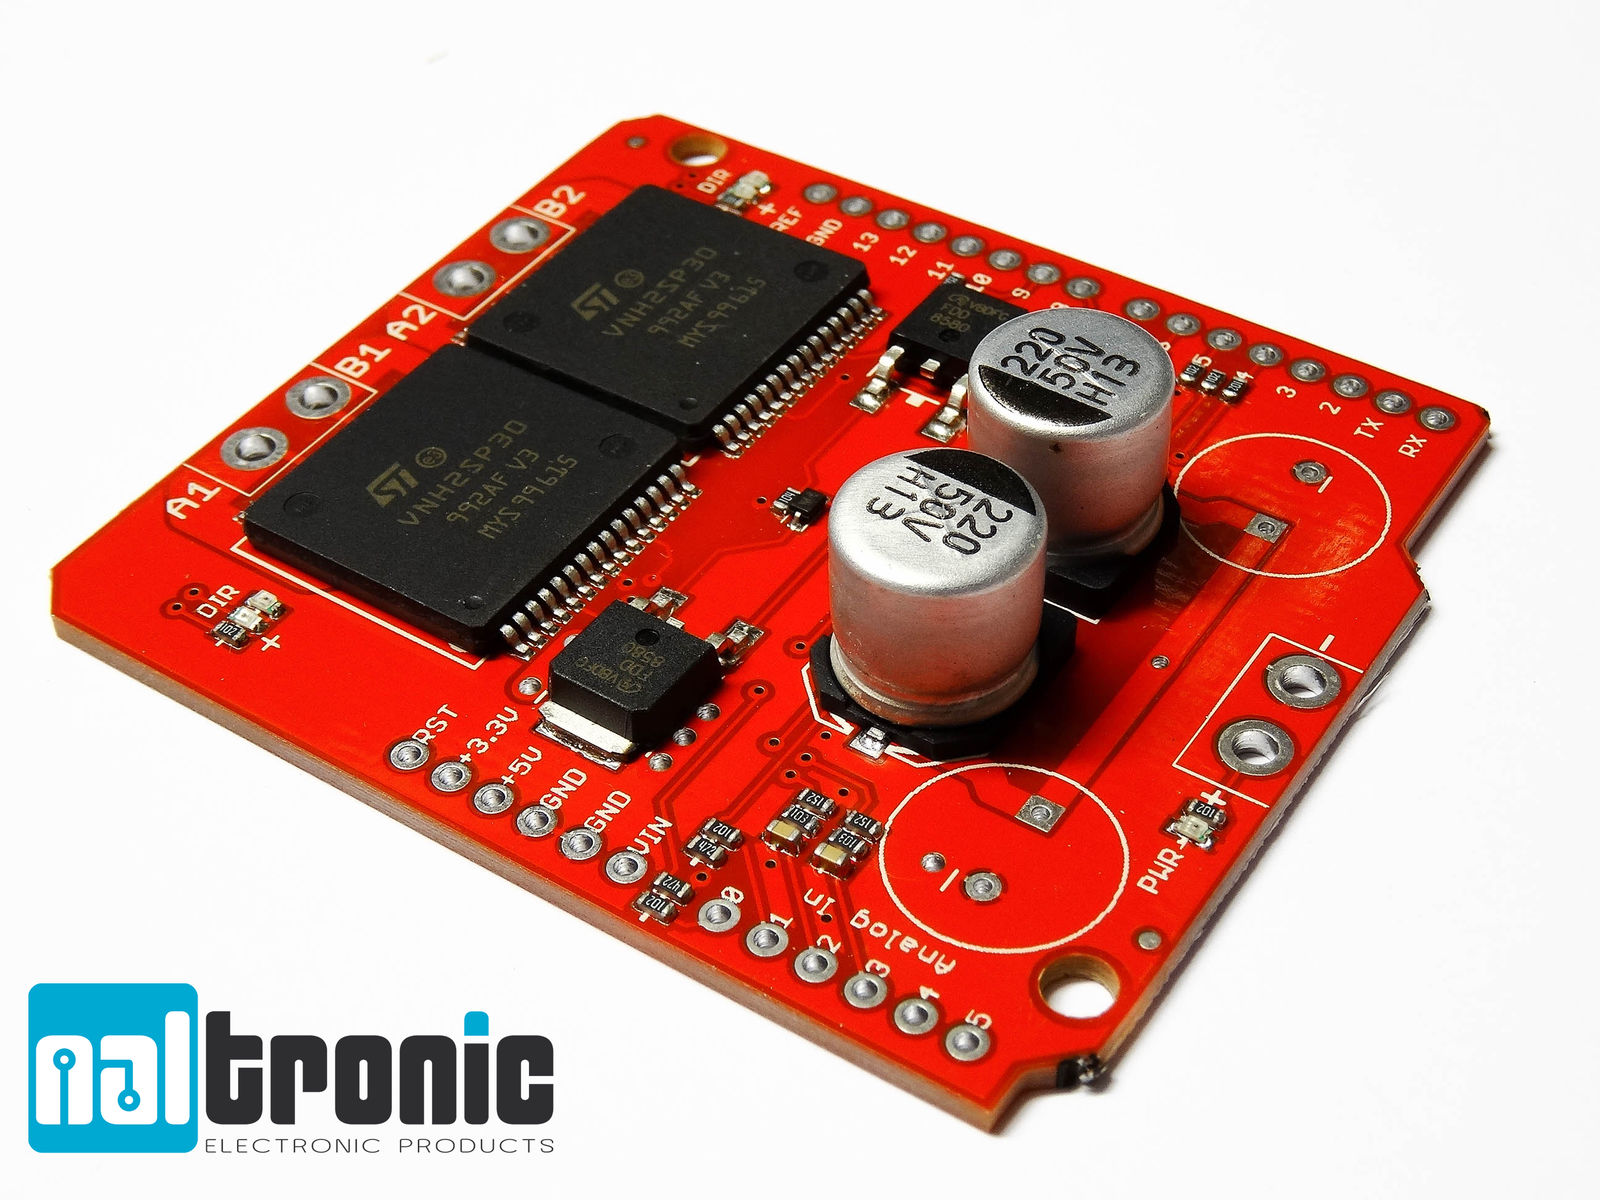
\includegraphics[width=10cm]{Bilder/Bauteile/Motorsteuerung}
\caption{Motorsteuerung}
\label{Motoransteuerung}

\end{center}
\end{figure}
Aus Sicherheits- und Kostentechnischen Gründen, wurde von einer manuell gesteuerten H-Brücke auf ein fertiges Motorsteuerungsmodul umgestiegen. Der Vorteil dieser Ansteuerung besteht darin, dass ein Kurzschluss der H-Brücke Hardwaretechnisch ausgeschlossen werden kann und damit nicht vond er Software abgesichert werden muss. Das Motormodul verfügt außerdem über eine Interne Strommessung für jeden der 2 unterstützten Motoren. Diese Messung kan bei bedarf abgefragt werden. Für unsere Anwendung ist dies jedoch nicht erforderlich. Der Mototreiber unterstützt 2 Motoren, welche mit bis zu 30 Ampere bei 16V betrieben werden können, bevor der IC überhitzt oder andere Bauteile zerstört werden. Die Ansteuerung jedes Motors erfolgt über ein Digitales Signal. Motor 1 kann über den Pin AI0 aktiviert(enabled) werden. Dies dient zur Sicherung das der Motor nicht ausversehen betätigt werden kann, solange der AI0 Pin nicht auf HIGH ist. Der enable Pin für Motor 2 ist AI1. Um Motor 1 in Uhrzeigersinn drehen zu lassen, muss der Pin D7 mit einem HIGH Signal und der Pin D8 mit einem LOW SIgnal angesteuert werden. Um Motor 2 gegen den Uhrzeigersinn drehen zu lassen, muss der Pin D8 mit einem HIGH Signal und der Pin D7 mit einem LOW Signal angesteuert werden. Um den Motor 1 bremsen zu können, muss Pin D8 und D7 mit entweder einem HIGH oder einem LOW Signal angesteuert werden. Für Motor 2 ist die Funktionsweise gleich jedoch muss der Pin D7 mit Pin D4 und Pin D8 mit Pin D9 ersetzt werden. Die externe Stromversorgung für den IC von 5V erfolgt über den VCC Pin. Die externe Stromversorgung für die Motoren erfolgt über den PWR Pin. Weiters muss der GND Pin noch mit einem der beiden Ground Anschlüsse der externen Stromversorgungen verbunden werden. Motor 1 wird über die Outputs A1 und B1 versorgt. Motor 2 wird über die Outputs A2 und B2 versorgt. Beim Anschluss der Motoren muss auf die Polung geachtet werdne und gegebenenfalls auch getestet werden, ob sich die Motoren auch wirklich beim Ansteuern der D7 oder D4 Pins in Uhrzeigersinn drehen und nicht gegen der Uhrzeigersinn. Falls beim Motor gekennzeichnet, sollte der Pluspol des Motors mit dem A1 beziehungsweise dem A2 Pin verbunden werden. Der Motortreiber verfügt auch über eine interne Drehzahlregelung, welche extra für beide Motoren über zwei PWM Input Pins gesteuert werden können. Die Drehzahl kann über den Duty Cycle des PWM Signals geregelt werden.
\subsubsection{PWM-Signal erzeugung für Motoransteuerung}
Ein PWM Signal ist ein periodisches Rechteck Signal. Eine Periode wird als Duty Cycle bezeichnet. Dieser Duty Cycle enthält eine Prozentangabe. Diese Prozentangabe sagt aus, wie viel Prozent des Duty Cycles HIGH und wie viel Prozent LOW sind. Ein Signal mit einem Duty Cycle von 100\% sagt aus, das eine Periodendauer zu 100\% aus einem HIGH Signal und zu 0\% aus einem LOW Signal besteht. Ein Duty Cycle von 25\% sagt aus, Das eine Periode zu 25\% aus einem HIGH Signal und zu 75\% aus einem LOW Signal besteht. Das PWM Signal kann von manchen ICs intern aufgenommen und der Duty Cycle ausgemessen werden. Dabei muss jedoch beachtet werden, dass die Frequenz des PWM Signals nicht die maximale Lesefrequenz des ICs übersteigt. Meistens wird diese Frequenz, wie bei unserem Motortreiber, im Datenblatt angegeben. Das PWM kann entweder über eigene ICs mit PWM Generatoren oder $\mu$Cs mit internen PWM Generatoren erzeugt werden. Das System muss nur über eine echtzeitfähigkeit besitzen, damit der Duty Cycle keine takte beim Zählen überspringen und damit nicht die frequenz fehlerhaft werden kann. 
Unser PWM Generator wurde mithilfe eines Arduino Nanos realisiert. Mithilfe des $\mu$C Atmega328P wird der Interne Zähler (Timer 2) dazu verwendet einen Output Pin in den richtigen Abständen zu toggeln (von HIGH auf LOW oder umgekehrt schalten) um ein PWM Signal zu erzeugen.


\begin{itemize}
\item verwendete Register:
\begin{itemize}
\item TCCR2A: Im TCCR2A Register wird festgelegt, in was für einem Modus der Timer laufen soll und was mit den Pins OC2A und OC2B passieren soll, wenn der der aktuelle Timer-Wert mit einem der beiden Output Compare Register übereinstimmt. Die Bits COM2A1 und COM2A0 setzen im Fast-PWM Modus fest, ob der OC2A Pin nicht beeinflusst wird und nicht verbunden ist, vom WGM22 Bit Abhängig ist, oder bei einem Compare Match, also wenn das Output Compare Register OCR2A mit dem Aktuellen Timer Wert übereinstimmt, der OC2A Pin gesetzt und beim reset des Timers resetet wird (non-inverting Mode), oder bei einem Compare Match der OC2A Pin resetet und beim reset des Timers gesetzt wird (inverting Mode). \\ Die selbe Funktion haben die Bits COM2B1 und COM2B0, nur dass der Pin OC2B verändert und mit dem Compare Registe OCR2B verglichen wird. \\
Die Bits WGM21 und WGM20 setzen den Modus des Signalgenerators die vom Timer unterstützt werden. Es gibt grundsätzlich 3 Modi in denen der Signalgenerator laufen kann: CTC, Fast PWM, PWM Phase Correct. \\
\begin{itemize}
\item Im CTC Modus kann der TOP Wert zu dem der Counter zählt, immer bei jedem vollständigen Zählvorgang geändert werden. Der Zähler zählt in Form eines Sägezahn Signals und toggled den Pin immer, wenn der Top Wert erreicht wird.\\
\item Im Fast PWM Modus zäjlt der Zähler in Form eines Sägezahnsignals und es wird bei jedem Zählschritt überprüft, ob der aktuelle Wert des Zählers mit dem Output Compare Register übereinstimmt. Was passiert, wenn die Werte übereinstimmen, wird in den COM2xx Bits festgelegt. Die Frequenz des Ausgangssignals am Pin kann nur über einen Prescaler verändert werden. Das bedeutet, dass die Frequenz nur 7 Frequenzen, mit dem internen Timer, annehmen kann. Das OCR2x Register kann während des betriebes geändert werden. Damit kann der Duty Cycle während des Betriebes geändert werden. \\
\item Der PWM Phase Correct Modus, lasst den Zähler von Bottom zu Top und wieder zu Bottom zählen. Das bewirkt, das er Zähler in Form eines Dreiecksignals zählt. Daher ist das Ausgangs PWM Signal immer symetrisch um den BOTTOM und TOP Wert des Zählers. Daher bleibt das Signal immer Phasenkorrekt. Der Nachteil dieses Modus ist, dass er nur die halbe Frequenz des Fast PWM Modus erreichen kann. Der PWM Phase Correct Modus, kann auch nur 7 Frequenzen annehmen.\\
\end{itemize} 
\item TCCR2B: Im TCCR2B Register wird für unsere Anwendung der Prescaler festgelegt um die frequenz des PWM-Signales einzustellen. Dazu werden die Bits 0 bis 2 verwendet. Das sind die Bits CS20, CS21 und CS22. Die Bits FOC2A, FOC2B und WGM22 werden in unserer Anwendung nicht benötigt und können ignoriert werden. \\
\item OCR2A: Das Register OCR2A ist das Output Compare Match Register für den OC2A Pin. Das Register kann einen Wert zwischen 0 und 255 haben wobei, im Fast PWM Modus, 0 einem Duty Cycle von 0\% und 255 einem Duty Cycle von 100\% entspricht.\\
\item OCR2B: Das Register OCR2B ist das Output Compare Match Register für den OC2B Pin. Das Register kann einen Wert zwischen 0 und 255 haben wobei, im Fast PWM Modus, 0 einem Duty Cycle von 0\% und 255 einem Duty Cycle von 100\% entspricht.\\
\item DDRD: Im Register DDRD können I/O Pins als Output Pins gesetzt werden. Es muss nur das Bit des entsprechenden Pins gesetzt werden.\\
\item DDRB: Im Register DDRB können I/O Pins als Output Pins gesetzt werden. Es muss nur das Bit des entsprechenden Pins gesetzt werden.\\
\end{itemize}
\item Frequenz berechnen:\\
Die maximal Frequenz des PWM-Signals für die Motoransteuerung beträgt 20kHz. Das bedeutet das man einen Frequenzwert so nahe wie mögliche, aber unter der Maximalen Frequenz wählen soll.\\
Berechnen lässt sich die Frequenz des PWM-Signals mit folgender Formel:
\begin{align*}
f_{OC2xPWM}=\frac{f_{clk\_I/O}}{N*256} \\
\end{align*} 
f$_{OC2xPWM}$ ist die Frequenz die das PWM-Signal haben wird.\\
f$_{clk_I/O}$ ist die Taktfrequenz des Atmega328P. Also 16MHz. \\
N ist der Wert des Prescalers, welcher im TCCR2B Register festgelegt wird. \\

\textbf{Frequenz berechnung:}\\
$f_{OC2xPWM}$=$\frac{f_{clk\_I/O}}{N*256}$ = $\frac{16000000}{8 \cdot 256}$ = $\underline{7812,5Hz}$
\item Programm für Atmega328P: \\
\begin{lstlisting}[caption=$\mu$C-Programm,language=c]
void app_main (void)
{
  DDRD = (1<<PD3);
  DDRB = (1<<PB3);
  TCCR2A = (1<<COM2A1) | (1<<COM2B1) | (1<<WGM21) | (1<<WGM20);
  TCCR2B = (1<<CS21);
  OCR2A = 0x5f;
  OCR2B = 0x5f;
  
}
\end{lstlisting}

\begin{itemize}
\item DDRD: Im DDRD Register wird der PD3 Pin auf Output geschaltet.\\
\item DDRB: Im DDRB Register wird der PB3 Pin auf Output geschaltet.\\
\item TCCR2A: Im TCCR2A Register wird der non-Inverting Fast-PWM Modus eingestellt für OC2A und OC2B. \\
\item TCCR2B: Im TCCR2B Register wird der Prescaler festgelegt. \\
\item OCR2A: Im OCR2A Register wird der Duty Cycle festgelegt. 0 entspricht 0\% und 255 entspricht 100\% \\
\item OCR2B: Im OCR2B Register wird der Duty Cycle festgelegt. 0 entspricht 0\% und 255 entspricht 100\% \\
\end{itemize}
\end{itemize}


\begin{figure}[H] 
\begin{center}

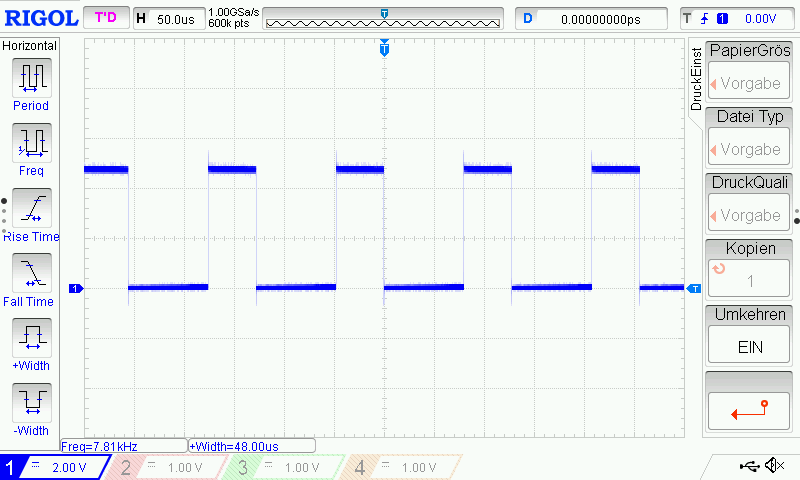
\includegraphics[width=15cm]{Bilder/PWM/pwm}
\caption{PWM}
\label{PWM}

\end{center}
\end{figure}
\newpage
\subsubsection{Gesamtschaltplan}
\begin{figure}[H] 
\begin{center}

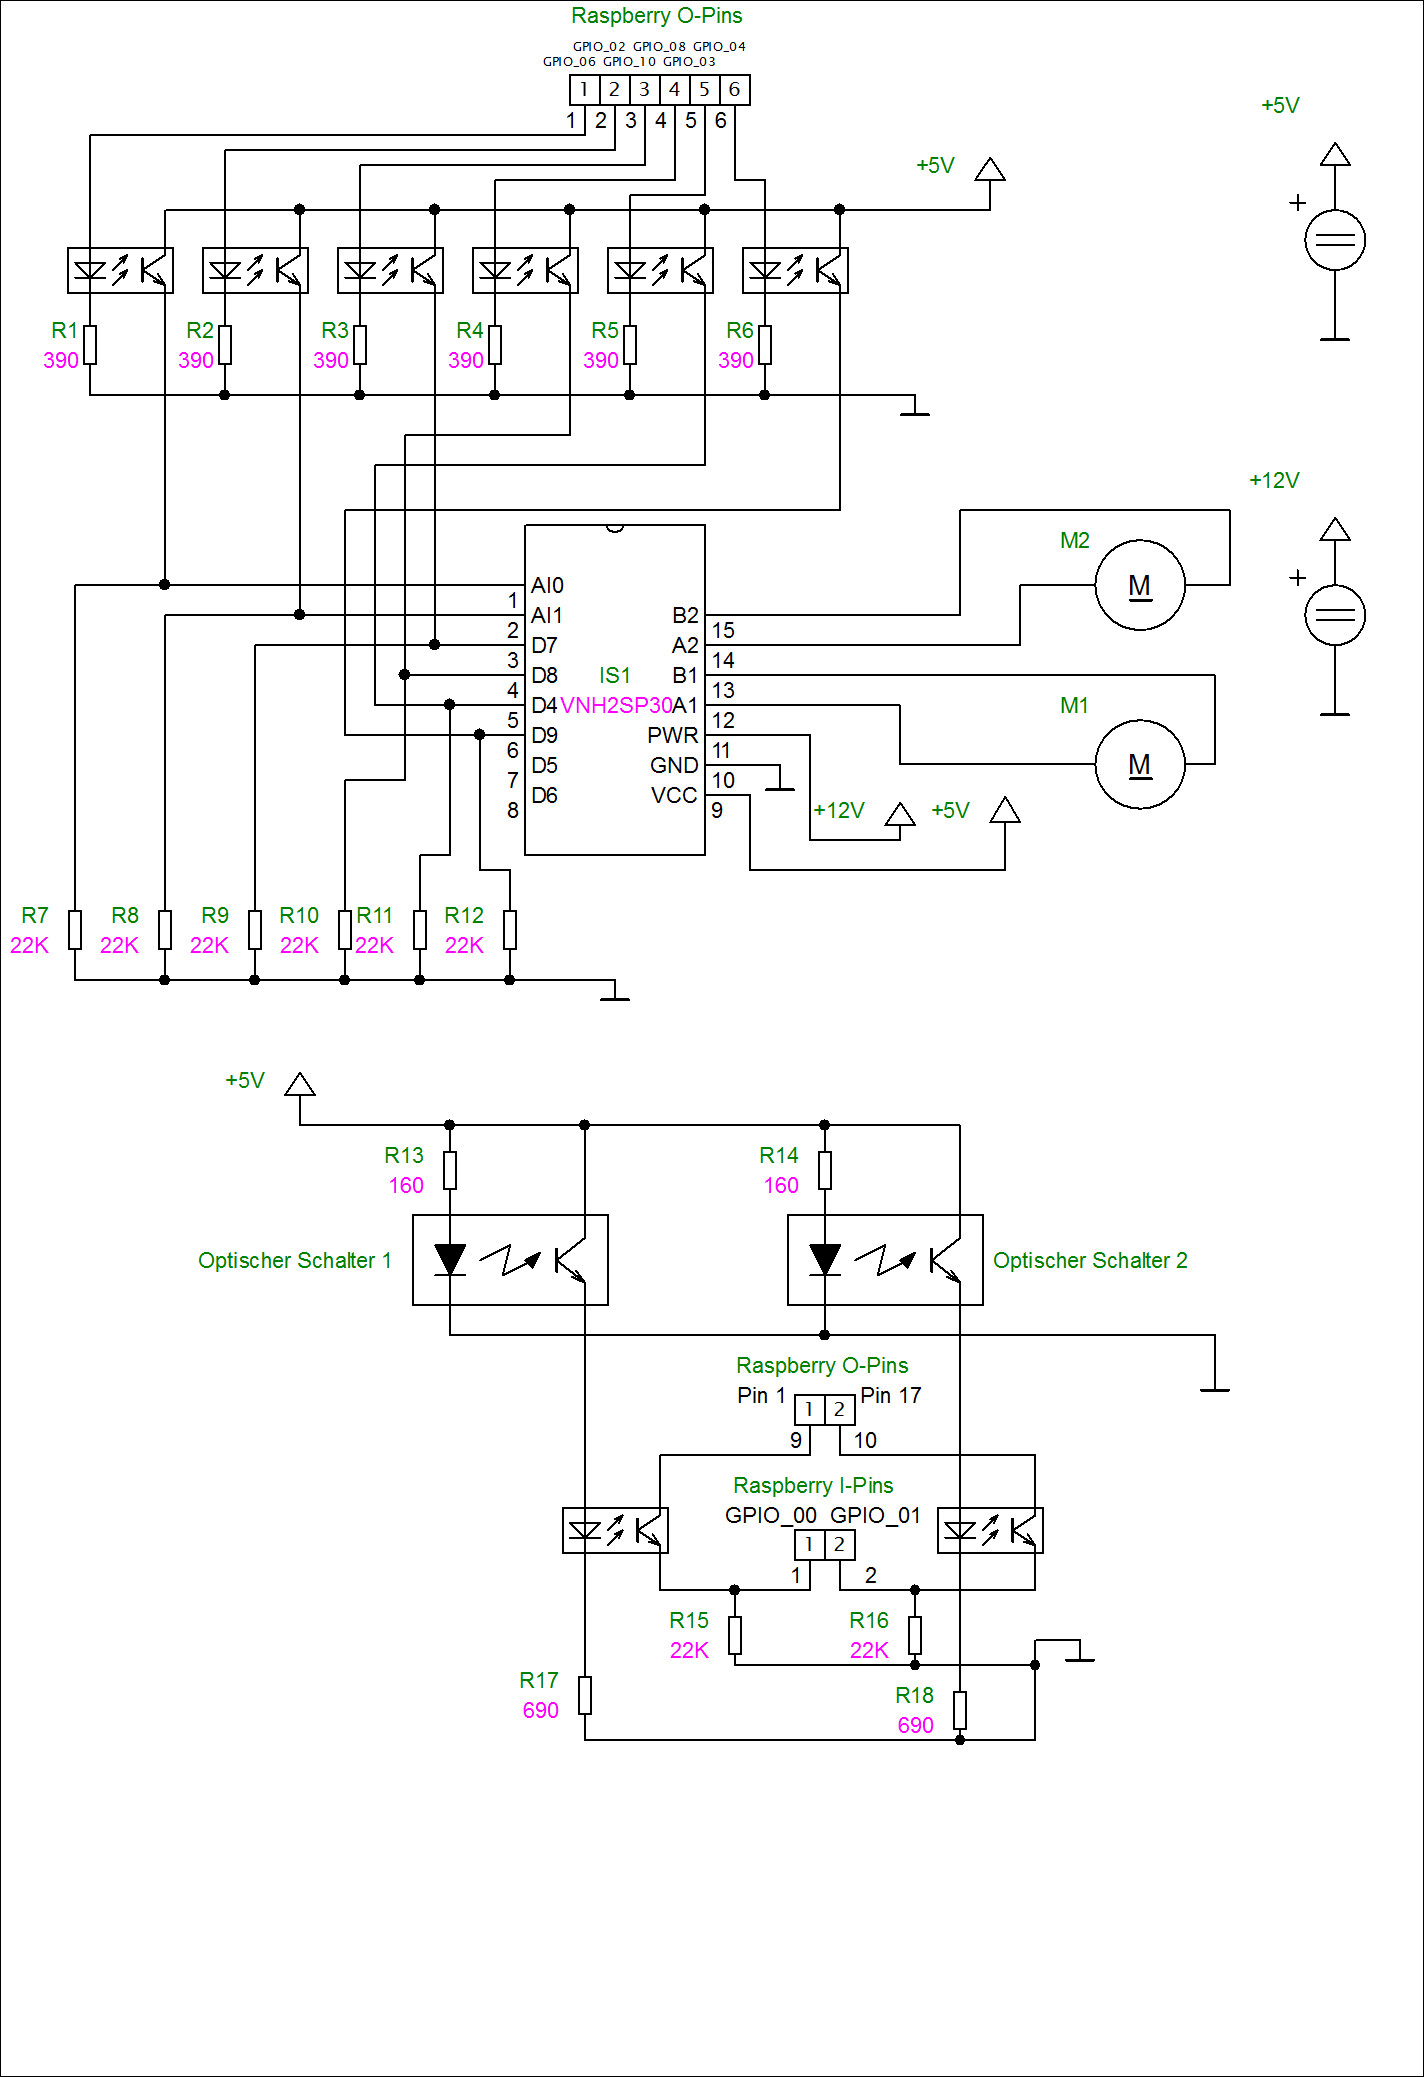
\includegraphics[width=15cm]{Bilder/Schaltplan/Gesamtschaltplan}
\caption{Gesamtschaltplan}
\label{Gesamtschaltplan}

\end{center}
\end{figure}
\subsubsection{Verkabelung der Motoransteuerung mit dazugehörigen Elementen}
\begin{figure}[H] 

\begin{center}

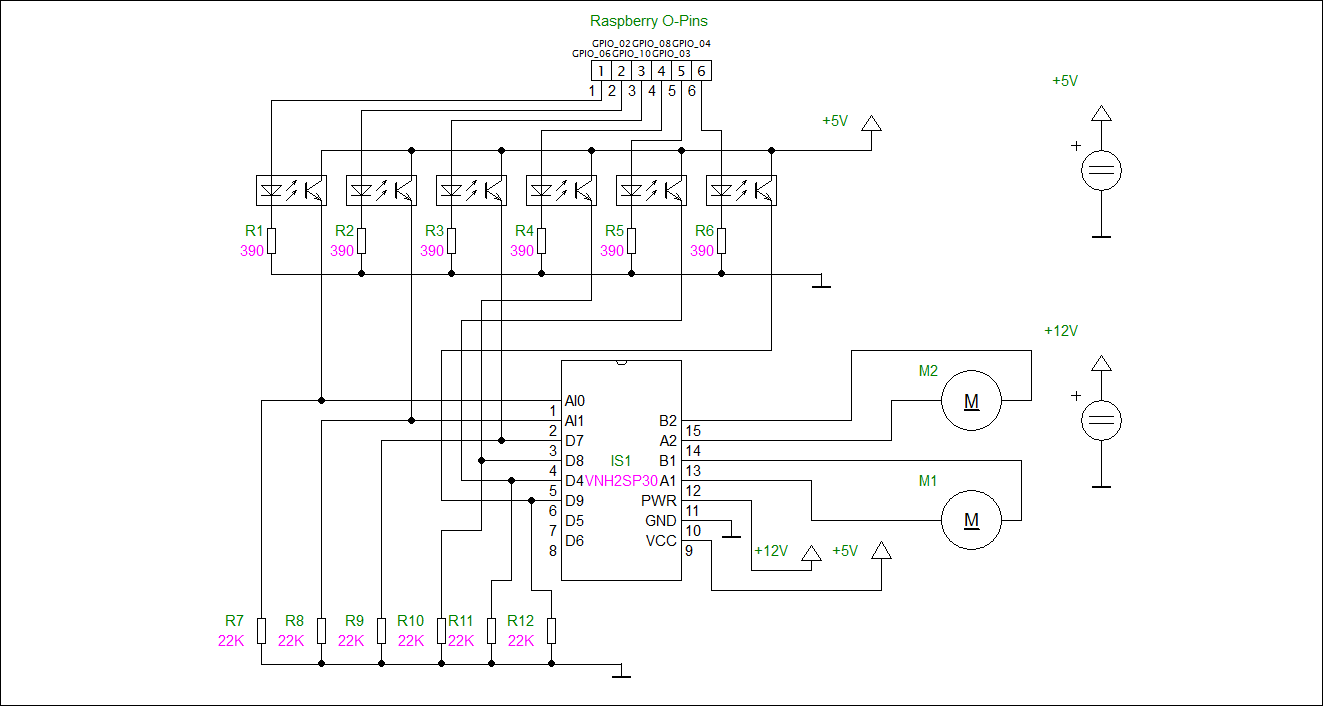
\includegraphics[width=15cm]{Bilder/Schaltplan/Motoransteuerung}
\caption{Motoransteuerung}
\label{Motoransteuerung}
\end{center}
\end{figure}
Die Motoransteuerung besteht aus folgenden Komponenten:\\
\begin{itemize}
\item Dem Motortreiber mit dem IC VNH2SP30.
\item Der Klemme Raspberry O-Pins, welche die GPIO-Pins des Raspberrys zur darstellung ersetzt.
\item Sechs Optokopplern, welche die Ausgangsspannung von den GPIO-Pins auf 5V bringt und die Raspberry-Pins vom restlichen Stromkreis galvanisch trennt.
\item Einem PWM-Generator in Form eines $\mu$Cs, welcher die Drehzahl der beiden Motoren steuert.
\item Den beiden Motoren M1 und M2.
\item Den Widerständen R1 bis R6, welche einen Spannungsabfall erzeugen, damit der Optokoppler nicht überlastet wird.
\item Den Pulldown-Widerständen R7 bis R12 welche ein floaten, also eine fehlerhafte Spannung an den Input-Pins der Motorsteuerung, verhindern sollen.
\item Den externen Spannungsversorgungen von 5V und 12V\\
\end{itemize}
\textbf{Genereller Ablauf:}
\begin{enumerate}
\item Der PWM Generator erzeugt ein Dauerhaftes PWM-Signal, welches an die PWM-Inputs D6 und D5 der Motoransteuerung gelegt wird.
\item Die GPIO-Pins geben ein High-Signal von 3,3V aus, welches die Optokoppler ansteuert. 
\item Der Optokoppler schaltet seinen internen Phototransistor durch und ermöglicht einen Stromfluss.
\item Dadurch, dass der Strom über die Optokoppler jetzt fließen kann, fließt ein Strom von der 5V Spannungsversorgung über den Optokpoppler in den Input-Pin der Motoransteuerung.
\item Je nach ansteuerung der Pins, dreht sich einer oder beide Motoren, in oder gegen den Uhrzeigersinn, oder werden gebremst. Dabei fließt ein Strom von der 12V Spannungsversorgung über die Motoransteuerung zu den Motoren.
\item Die Motoransteuerung regelt die Spannung an den Motoren mittels des PWM-Signals und regelt auch die Drehrichtung der Motoren je nach ansteuerung.
\end{enumerate}
\textbf{Berechnungen:}
\begin{itemize}
\item R1 bis R6: \\
Die Spannung die abfallen muss, und der Strom der fließt, kann aus dem Datenblatt des Optokopplers entnommen werden.\\
$U_{Optokoppler}=$1,15V \\
$U_{Optokoppler-max}=$1,4V \\
$I_{Optokoppler}$=5mA \\

\begin{center}
$R_{1,2,3,4,5,6}=\frac{U}{I}=\frac{U_{GPIO}-U_{Optokoppler}}{I_{Optokoppler}}=\frac{3,3V-1,15V}{0,005A}=430\Omega$
\end{center}
Da 430$\Omega$ kein E12-Wert ist, wird ein 390$\Omega$ Widerstand hergenommen.
Zur überprüfung, ob dieser Wert angenommen werden kann, muss die Spannung am Optokoppler neu gerechnet und überprüft werden, ob die Spannung zwischen der maximal zuläassige und der normalen Spannung ist.
\begin{center}
$U_{Optokoppler}=U_{GPIO}-(R_{1,2,3,4,5,6} \cdot I_{optokoppler})=3,3V-(390\Omega \cdot 0,005A) = 1,35V < U_{Optokoppler-max}$
\end{center}
Da die tatsächliche Spannung zwischen der maximalen und normalen Spannung des Optokopplers ist, ist dieser Widerstandswert zulässig.\\
\item R7 bis R12:\\
Diese Widerstandswerte werden mit 22k$\Omega$ angenommen.
\end{itemize}

\subsubsection{Verkabelung des Sensors mit dazugehörigen Elementen} 
\begin{figure}[H] 
\begin{center}

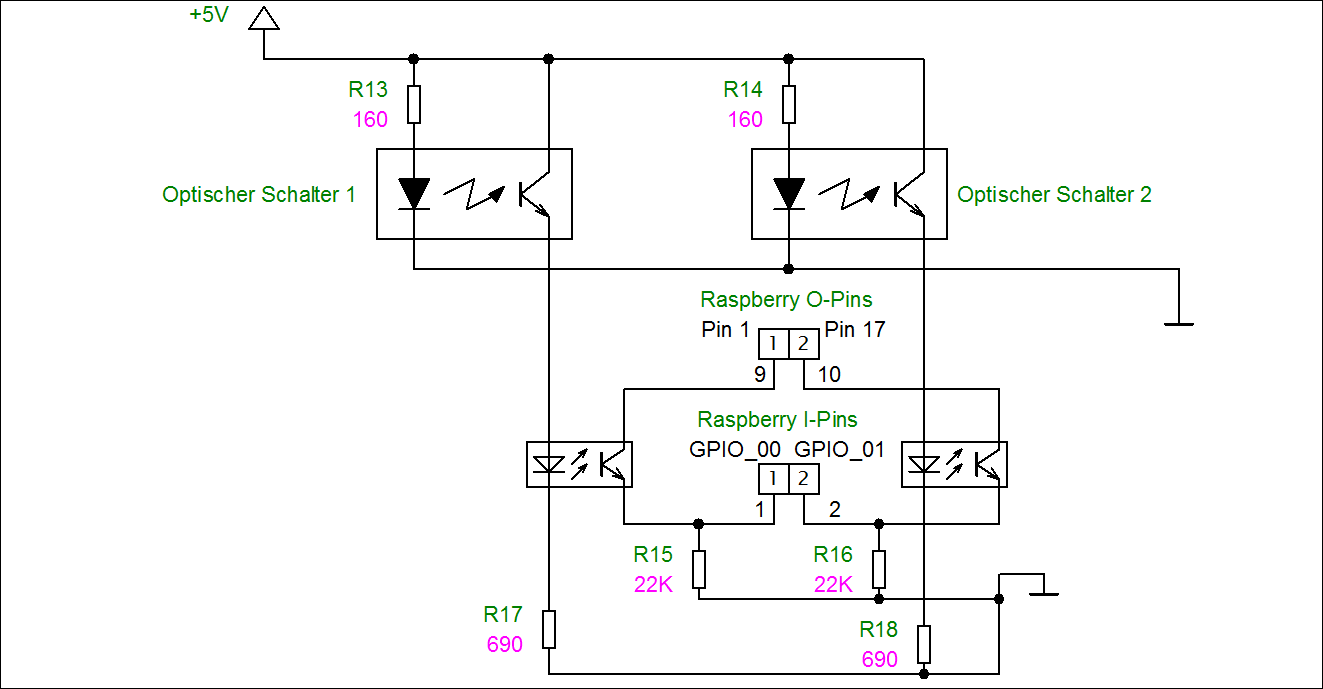
\includegraphics[width=15cm]{Bilder/Schaltplan/Sensoransteuerung}
\caption{Sensoransteuerung}
\label{Sensoransteuerung}

\end{center}
\end{figure}

Die Sensoransteuerung besteht aus folgenden Komponenten:
\begin{itemize}
\item Den optischen Sensoren OPB732WZ.
\item Der Klemme Raspberry O-Pins, welche die 3,3V-Pins des Raspberrys zur darstellung ersetzt.
\item Der Klemme Raspberry I-Pins, welche die GPIO-Pins des Raspberrys zur darstellung ersetzt.
\item Zwei Optokopplern, welche die Spannung der Sensoren von 5V auf ein 3,3V Potenzial bringen.
\item Den Widerständen R13 und R14, welche einen Spannungsabfall erzeugen, damit der Sensor nicht überlastet wird.
\item Den Widerständen R17 und R18, welche einen Spannungsabfall erzeugen, damit der Optokoppler nicht überlastet wird.
\item Den Pulldown-Widerständen R15 und R16 welche ein floaten, also eine fehlerhafte Spannung an den Input-Pins des Raspberrys, verhindern sollen.
\item Der externen Spannungsversorgunge von 5V\\
\end{itemize}
\textbf{Genereller Ablauf:}
\begin{enumerate}
\item Wenn der Sensor eine Reflektor-Fläche vor sich erkennt, schaltet der Phototransistor im Sensor durch.
\item Der durchgeschaltete Phototransistor, ermöglich einen Stromfluss von der Spannunsguelle in den Optokoppler.
\item Dadurch schaltet der interne Phototransistor des Optokopplers durch.
\item Der durchgeschaltete Phototransistor, ermöglich einen Stromfluss von einem der 3,3V-Pins in einen der GPIO-Pins des Raspberrys.
\item Somit kann erkannt werden, welcher der Sensoren eine Reflektor-Fläche erkennt und weitere Softwaretechnische Maßnahmen können erfolgen.
\end{enumerate}
\textbf{Berechnungen:}
\begin{itemize}
\item R17 und R18: \\
Die Spannung die abfallen muss, und der Strom der fließt, kann aus den Datenblättern des Sensors und des Optokopplers entnommen werden.\\
$U_{Optokoppler}=$1,15V \\
$U_{Optokoppler-max}=$1,4V \\
$U_{CE(SAT)}=$0,4V \\
$I_{Optokoppler}$=5mA \\

\begin{center}
$R_{13,14}=\frac{U}{I}=\frac{U_{5V}-U_{Optokoppler}-U_{CE(SAT)}}{I_{Optokoppler}}=\frac{5V-1,15V-0,4V}{0,005A}=690\Omega$
\end{center}
Da 690$\Omega$ kein E12-Wert ist, wird ein 680$\Omega$ Widerstand hergenommen.
Zur überprüfung, ob dieser Wert angenommen werden kann, muss die Spannung am Optokoppler neu gerechnet und überprüft werden, ob die Spannung  zwischen der maximal zuläassige und der normalen Spannung ist.
\begin{center}
$U_{Optokoppler}=U_{5V}-U_{CE(SAT)}-(R_{13,14} \cdot I_{optokoppler})=5V-0,4V-(680\Omega \cdot 0,005A) = 1,2V => U_{Optokoppler} < 1,2V < U_{Optokoppler-max}$
\end{center}
Da die tatsächliche Spannung zwischen der maximalen und normalen Spannung des Optokopplers ist, ist dieser Widerstandswert zulässig.\\
\item R13 und R14:\\
Die Spannung die abfallen muss, und der Strom der fließt, kann aus dem Datenblatt des Sensors entnommen werden.\\
$U_{F}=$1,8V \\
$I_{F}$=20mA \\

\begin{center}
$R_{13,14}=\frac{U}{I}=\frac{U_{5V}-U_{F}}{I_{F}}=\frac{5V-1,8V}{0,02A}=160\Omega$
\end{center}
Da 160$\Omega$ kein E12-Wert ist, wird ein 180$\Omega$ Widerstand hergenommen.
Zur überprüfung, ob dieser Wert angenommen werden kann, muss die Spannung am Optokoppler  neu gerechnet werden und überprüft werden, ob die Spannung geringer als die maximal zuläassige Spannung ist.
\begin{center}
$U_{F}=U_{5V}-(R_{13,14} \cdot I_{F})=5V-(180\Omega \cdot 0,02A) = 1,4V$
\end{center}
Da 1,4V die Spannung U$_{F}$ zu sehr unterschreiten würde, wird eine Seriellschaltung von einem 150$\Omega$ und einem 10$\Omega$ Widerstand benötigt.
\item R15 und R16:\\
Diese Widerstandswerte werden mit 22k$\Omega$ angenommen.
\end{itemize}

\section{Mechanische Konstruktion}
\subsection{Motorhalterung Futterschüsseldrehplatte}
\subsection{Motorhalterung Förderband}
\subsection{Sensorhalterung Futterschüsseldrehplatte}
\subsection{Sensorhalterung Förderband}
\subsection{Halterung Raspberry und $\mu$C}
\subsection{Lüfterhalterung für Raspberry}
\newpage
\section{Stückliste}
\begin{tiny}
\begin{center}
\begin{tabular}{|p{2cm}|c|c|p{3cm}|p{7cm}|} \hline
Name & ID & Stückzahl & Anmerkung & Link \\ \hline
Optek Optischer Näherungsschalter & OPB732WZ & 2 & - & \url{https://at.rs-online.com/web/p/products/9087113/?gclid=Cj0KCQjw6NjNBRDKARIsAFn3NMq0RvGj3r_5q7xtFIs2eGGmyLAENp-a446vhWDjUIsFB9L3bRjBDXUaAqj1EALw_wcB&cm_mmc=AT-PLA-DS3A-_-google-_-PLA_AT_DE_Automation-_-Sensoren_Und_Messwandler-_-PRODUCT+GROUP&matchtype=&grossPrice=Y&gclsrc=aw.ds} \\ \hline 
Optokoppler & SFH6916 & 2 & 4 Optokoppler pro Bauteil & \url{https://www.neuhold-elektronik.at/catshop/product_info.php?products_id=4181} \\ \hline
Motorsteuerung & VNH2SP30 & 1 & Fertiges Modul aus 2 ICs und zusätzlicher Beschaltung & \url{https://www.ebay.at/itm/30A-VNH2SP30-Dual-Stepper-Motor-Driver-Monster-Moto-Shield-Module-Motortreiber/122543212784?hash=item1c882508f0:g:QGkAAOSwsy9amWPw} \\ \hline
Gleichstrom Motor & FD MY2007 U222 60x & 2 & Schneckengetriebe & \url{https://www.neuhold-elektronik.at/catshop/product_info.php?cPath=96_99&products_id=5522} \\ \hline
Schaltnetzteil 5V & ASTEC LPS42 & 1 & 11A & \url{https://www.neuhold-elektronik.at/catshop/product_info.php?cPath=114_118&products_id=6596} \\ \hline
Schaltnetzteil 12V & - & 1 & 30A & \url{https://www.optonicaled.at/netzeil-metal-360w?gclid=Cj0KCQjwv73VBRCdARIsAOnG8u3XQ-am7_9sgk8srkL6hS7SgxZRm4DZmOgQmx8V2TWz59MP70Hgx7QaAjuqEALw_wcB} \\ \hline
Lüfter 12V & EE80251S2-0000-999 & 1 & 80x80x25mm & \url{https://www.conrad.at/de/axialluefter-12-vdc-6286-mh-l-x-b-x-h-80-x-80-x-25-mm-sunon-ee80251s2-0000-999-323905.html} \\ \hline
Widerstand & - & 6 & Kohleschicht 390$\Omega$ & \url{https://www.conrad.at/de/kohleschicht-widerstand-390-axial-bedrahtet-0204-01-w-5-tru-components-1-st-1557169.html} \\ \hline
Widerstand & - & 2 & Kohleschicht 150$\Omega$ & \url{https://www.conrad.at/de/kohleschicht-widerstand-150-axial-bedrahtet-0204-01-w-5-1-st-400157.html} \\ \hline
Widerstand & - & 2 & Kohleschicht 10$\Omega$ & \url{https://www.conrad.at/de/kohleschicht-widerstand-10-axial-bedrahtet-0207-025-w-5-yageo-cfr-25jt-52-10r-1-st-1417641.html} \\ \hline
Widerstand & - & 2 & Kohleschicht 680$\Omega$ & \url{https://www.conrad.at/de/kohleschicht-widerstand-680-axial-bedrahtet-0207-025-w-5-yageo-cfr-25jt-52-680r-1-st-1417677.html} \\ \hline
Widerstand & - & 8 & Kohleschicht 22k$\Omega$ & \url{https://www.conrad.at/de/kohleschicht-widerstand-22-k-axial-bedrahtet-0207-025-w-5-yageo-cfr-25jt-52-22k-1-st-1417666.html} \\ \hline
Arduino Nano & - & 1 & Atmega328P zur PWM generierung & \url{https://www.amazon.de/AptoFun-Org-ATmega328P-FT232RL-Development-kompatibel/dp/B014TE52RS/ref=sr_1_1_sspa?ie=UTF8&qid=1521579402&sr=8-1-spons&keywords=arduino+nano&psc=1} \\ \hline
\end{tabular}
\end{center}
\end{tiny}